\subsection{Comparação entre o porte e o jogo original}

Esta seção tem como objetivo comparar resultado final do porte do jogo com o jogo original. O jogo portado para GBA pode ser encontrado no seguinte endereço: \url{https://github.com/traveling-will-gba/gbengine/tree/dev/test/game}.

\clearpage

\begin{figure}%
    \centering
    \subfloat[Menu original. Fonte: \textit{Autores}.]{{\includegraphics[width=12cm]{figuras/comparacao/pc-menu.eps} }}%
    \qquad
    \subfloat[Menu portado. Fonte: \textit{Autores}.]{{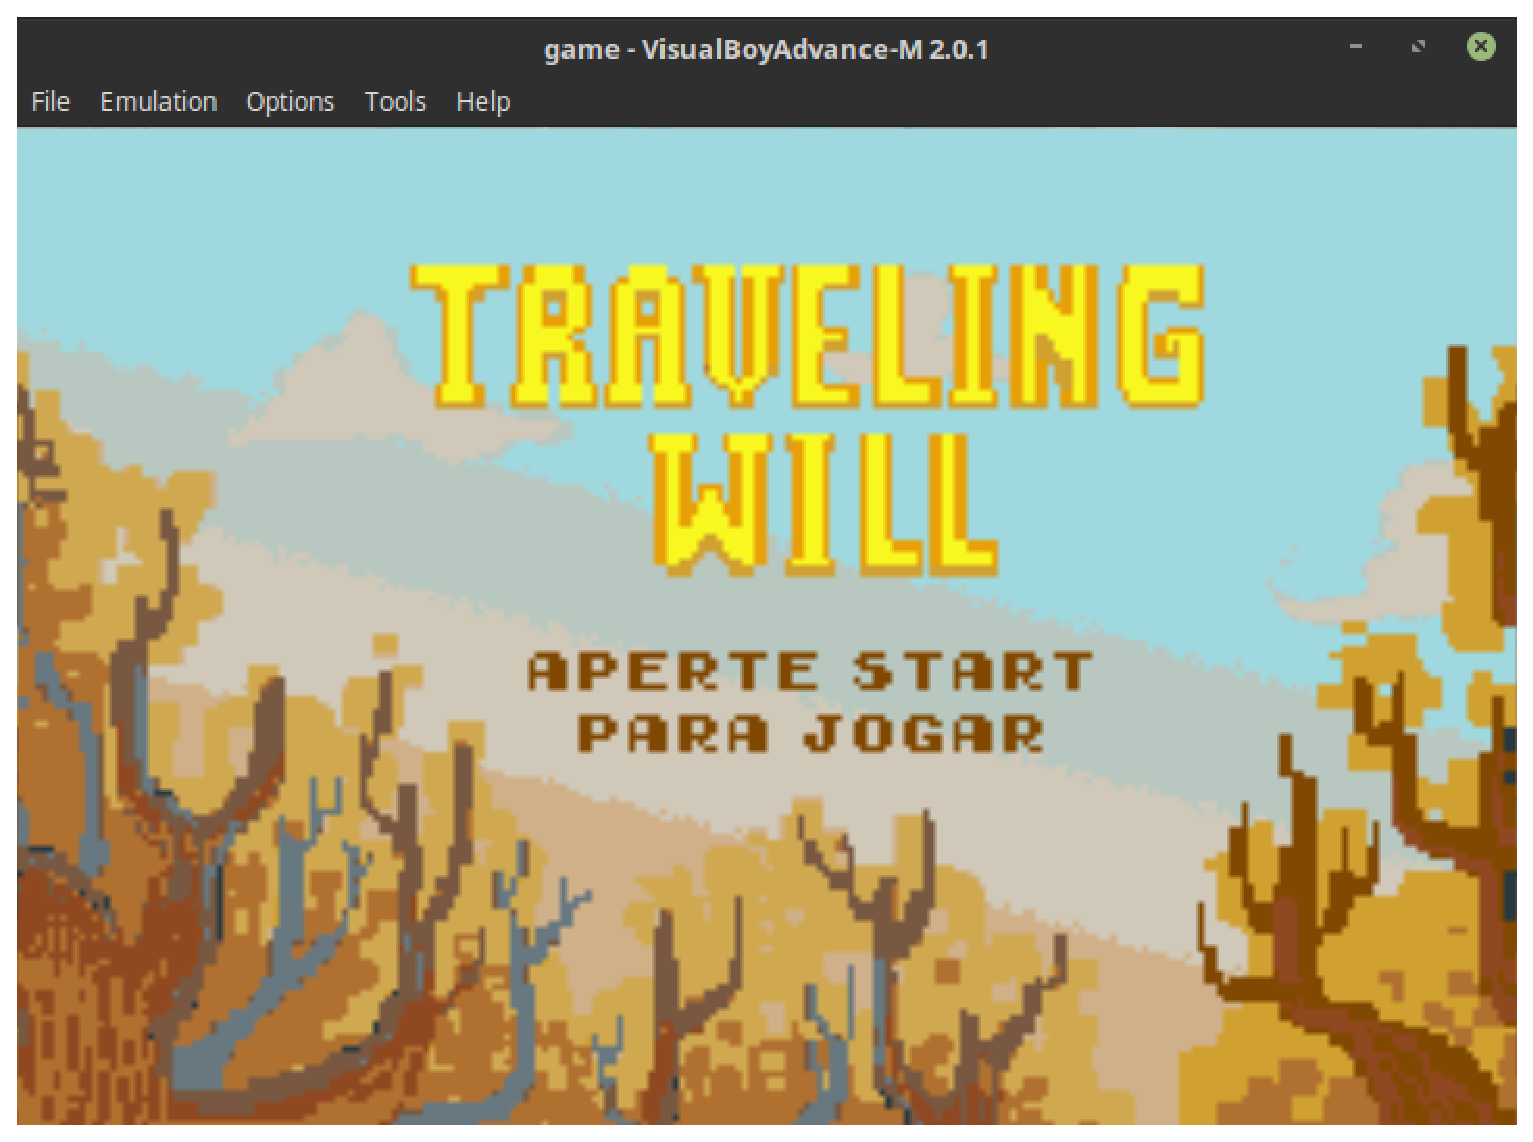
\includegraphics[width=12cm]{figuras/comparacao/gba-menu.eps} }}%
    \caption{Comparação do menu principal.}%
    \label{fig:example}%
\end{figure}

\begin{figure}%
    \centering
    \subfloat[Primeira fase original. Fonte: \textit{Autores}.]{{\includegraphics[width=12cm]{figuras/comparacao/pc-fase1.eps} }}%
    \qquad
    \subfloat[Primeira fase portada. Fonte: \textit{Autores}.]{{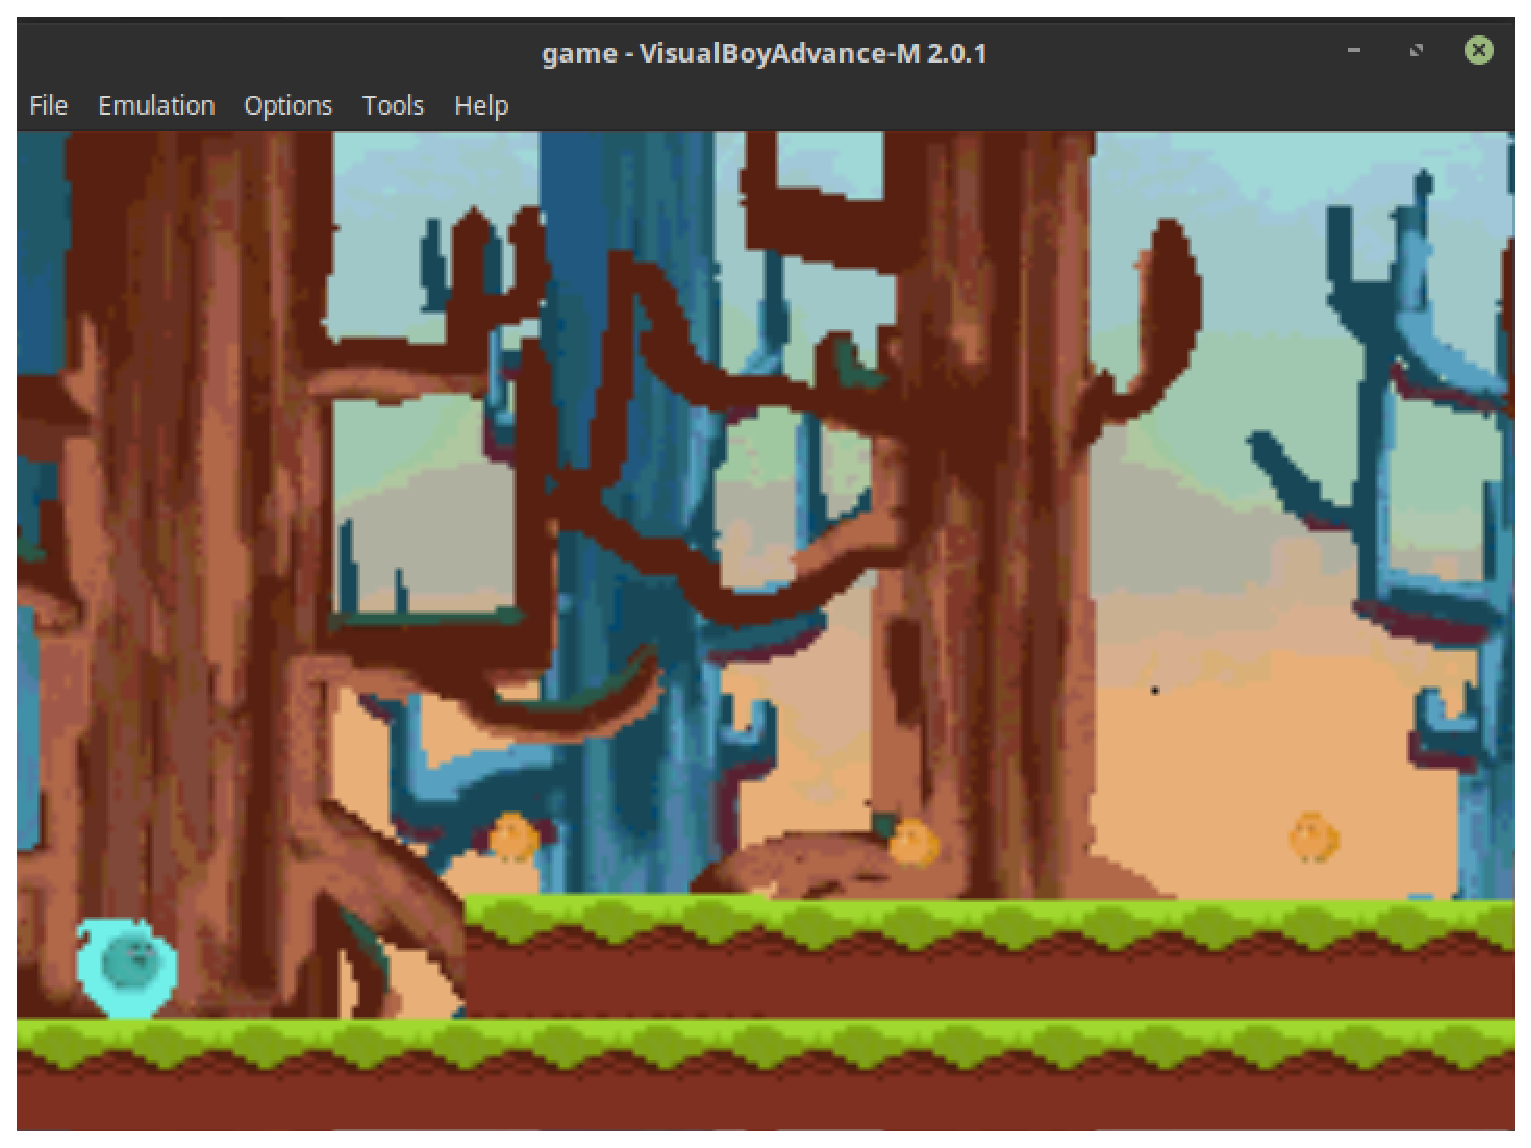
\includegraphics[width=12cm]{figuras/comparacao/gba-fase1.eps} }}%
    \caption{Comparação da primeira fase.}%
    \label{fig:example}%
\end{figure}

\begin{figure}%
    \centering
    \subfloat[Segunda fase original. Fonte: \textit{Autores}.]{{\includegraphics[width=12cm]{figuras/comparacao/pc-fase2.eps} }}%
    \qquad
    \subfloat[Segunda fase portada. Fonte: \textit{Autores}.]{{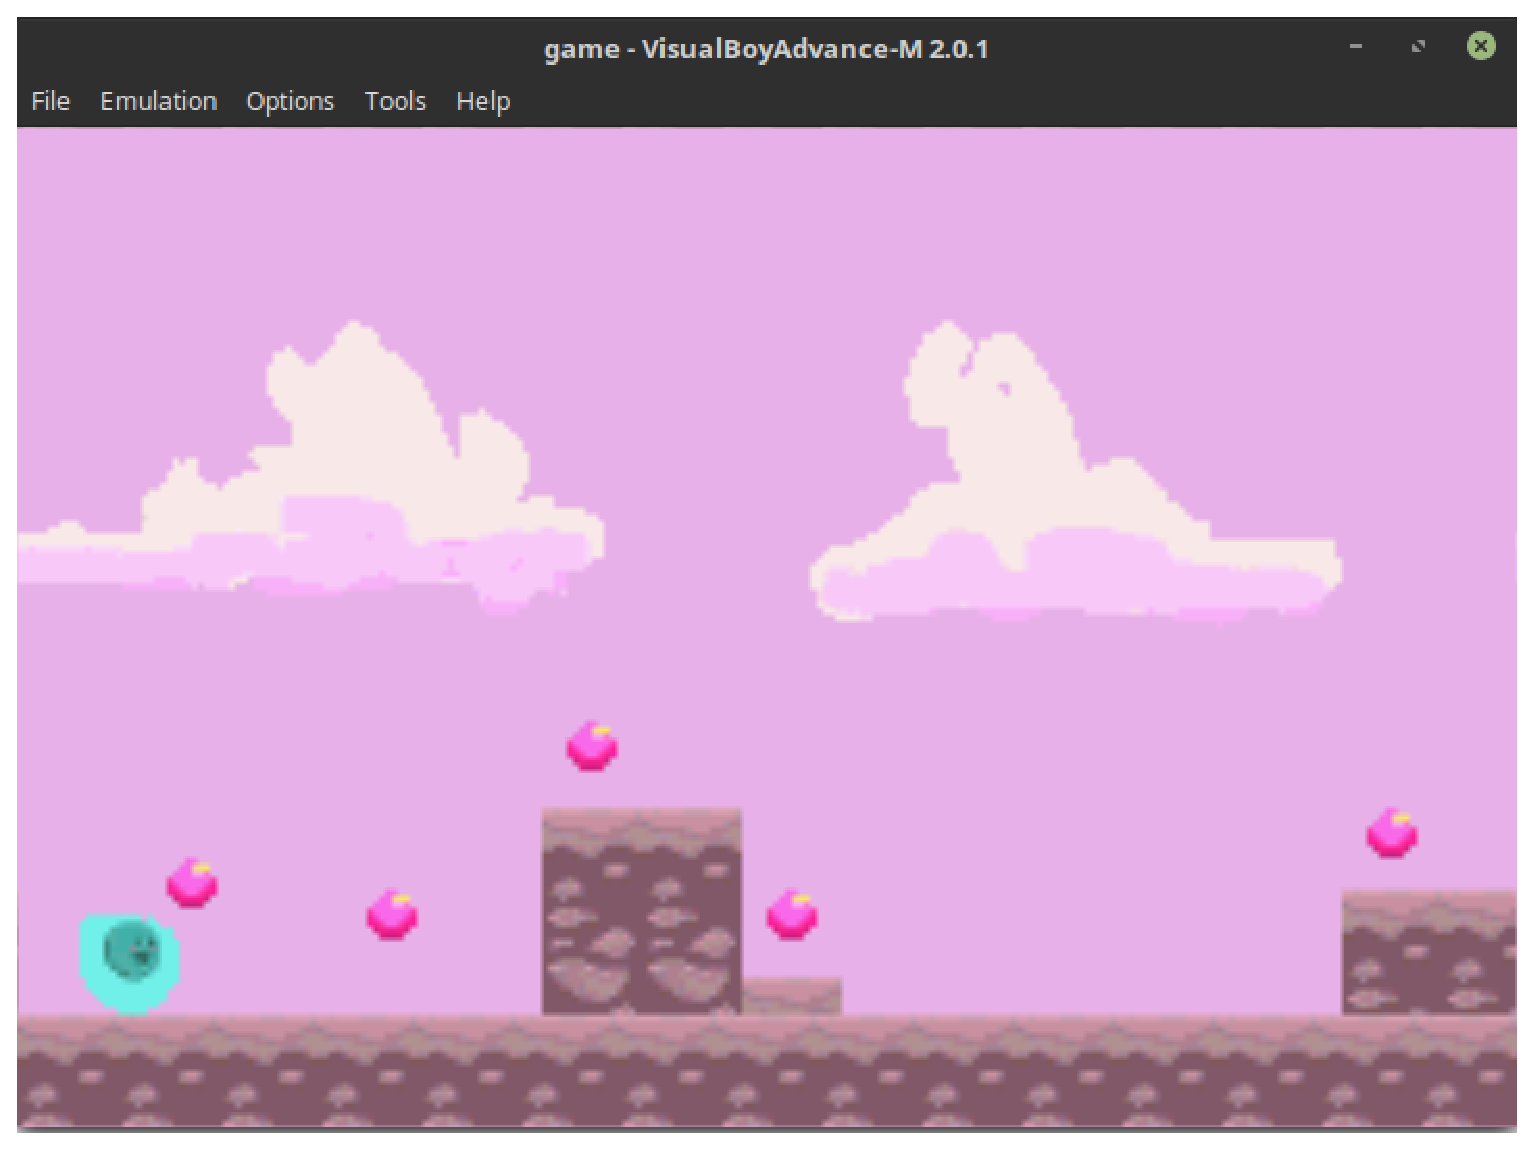
\includegraphics[width=12cm]{figuras/comparacao/gba-fase2.eps} }}%
    \caption{Comparação da segunda fase.}%
    \label{fig:example}%
\end{figure}

\begin{figure}%
    \centering
    \subfloat[Terceira fase original. Fonte: \textit{Autores}.]{{\includegraphics[width=12cm]{figuras/comparacao/pc-fase3.eps} }}%
    \qquad
    \subfloat[Terceira fase portada. Fonte: \textit{Autores}.]{{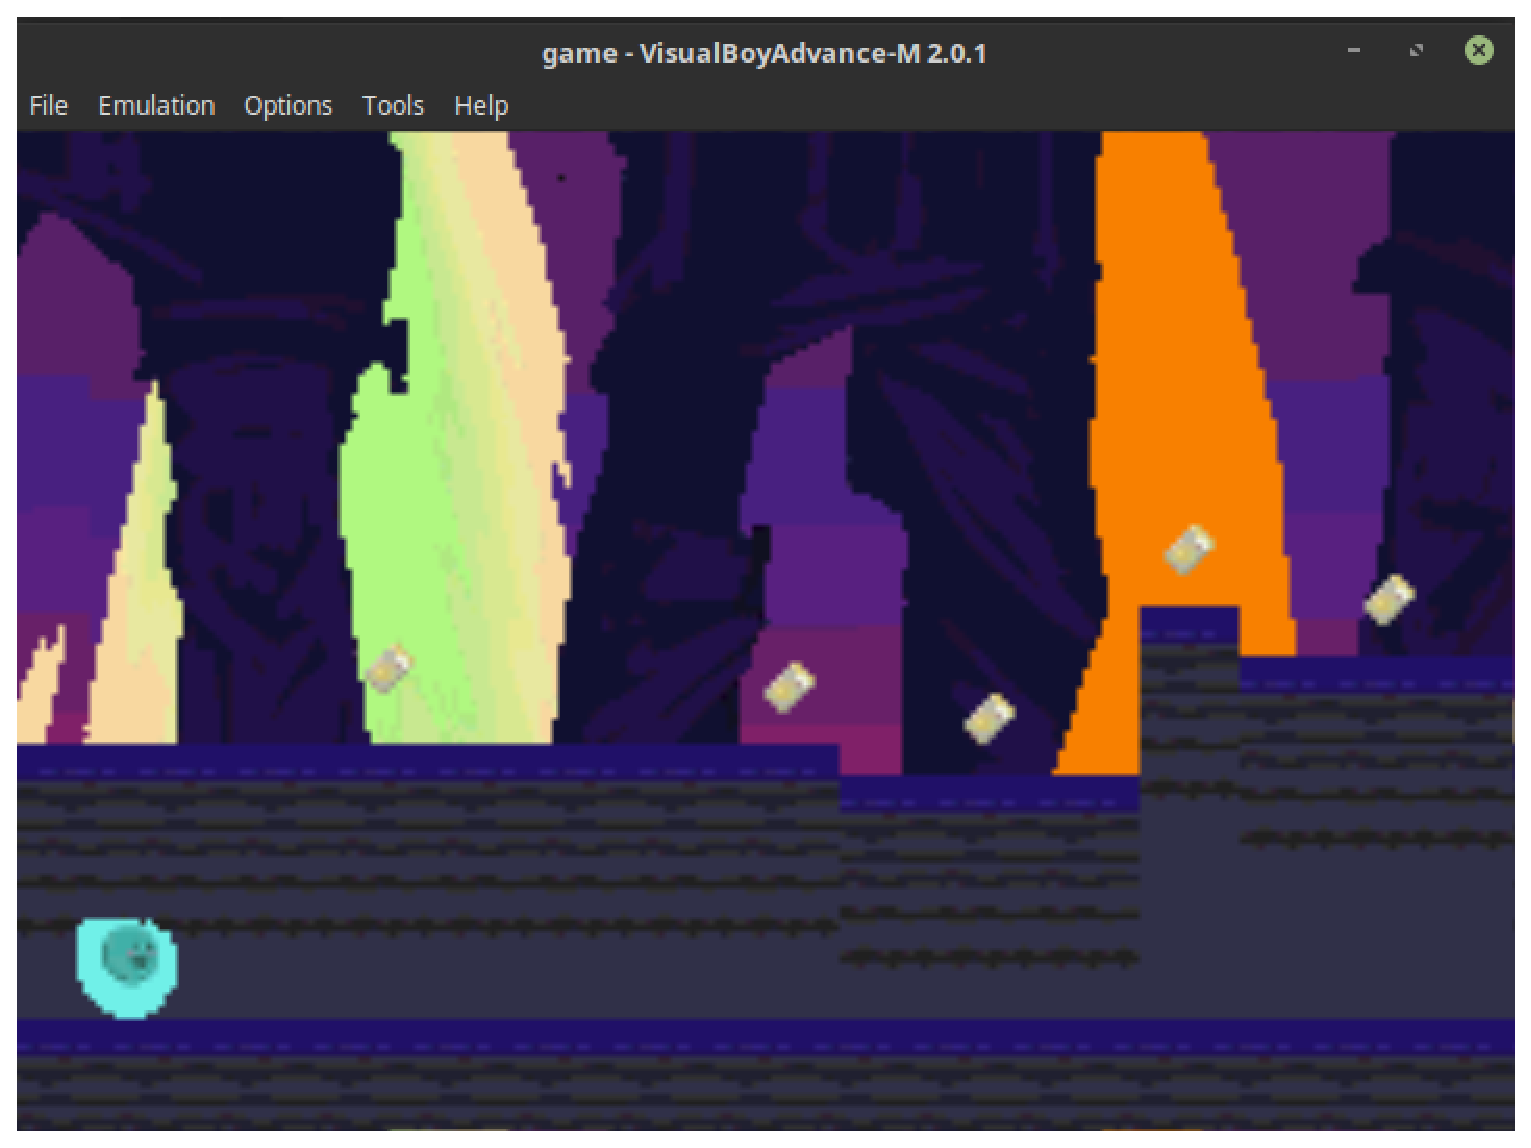
\includegraphics[width=12cm]{figuras/comparacao/gba-fase3.eps} }}%
    \caption{Comparação da terceira fase.}%
    \label{fig:example}%
\end{figure}

\begin{figure}%
    \centering
    \subfloat[Quarta fase original. Fonte: \textit{Autores}.]{{\includegraphics[width=12cm]{figuras/comparacao/pc-fase4.eps} }}%
    \qquad
    \subfloat[Quarta fase portada. Fonte: \textit{Autores}.]{{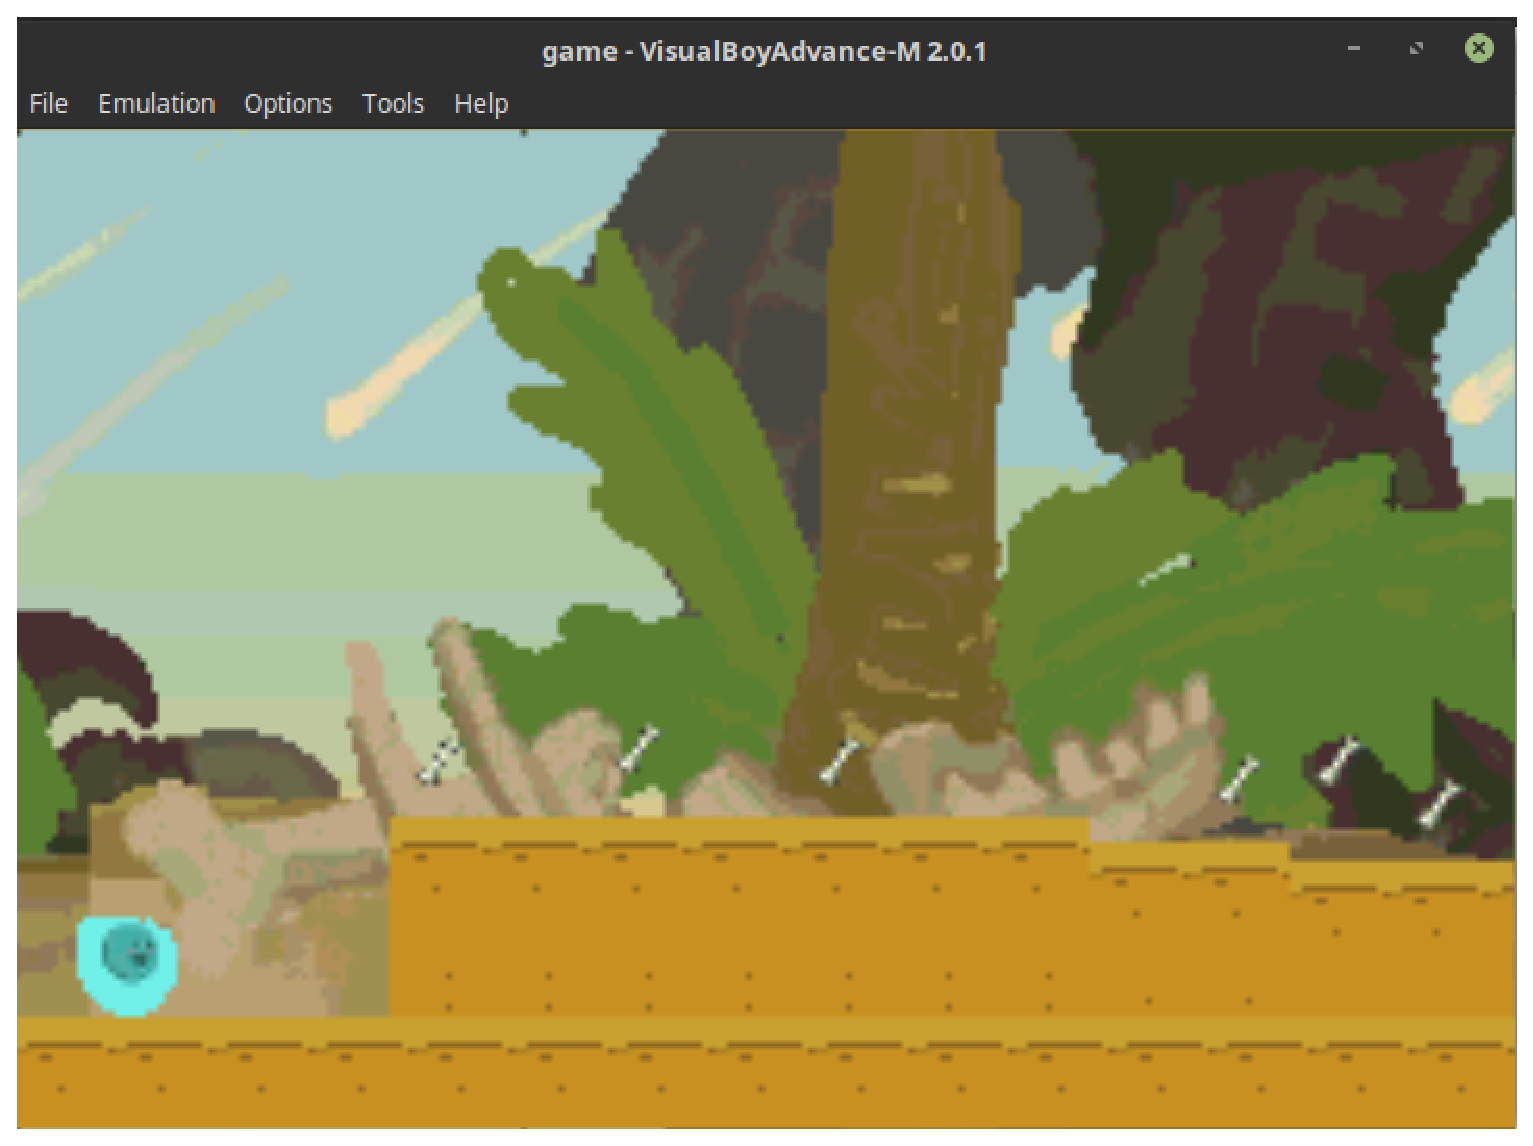
\includegraphics[width=12cm]{figuras/comparacao/gba-fase4.eps} }}%
    \caption{Comparação da quarta fase.}%
    \label{fig:example}%
\end{figure}

\begin{figure}%
    \centering
    \subfloat[Quinta fase original. Fonte: \textit{Autores}.]{{\includegraphics[width=12cm]{figuras/comparacao/pc-fase5.eps} }}%
    \qquad
    \subfloat[Quinta fase portada. Fonte: \textit{Autores}.]{{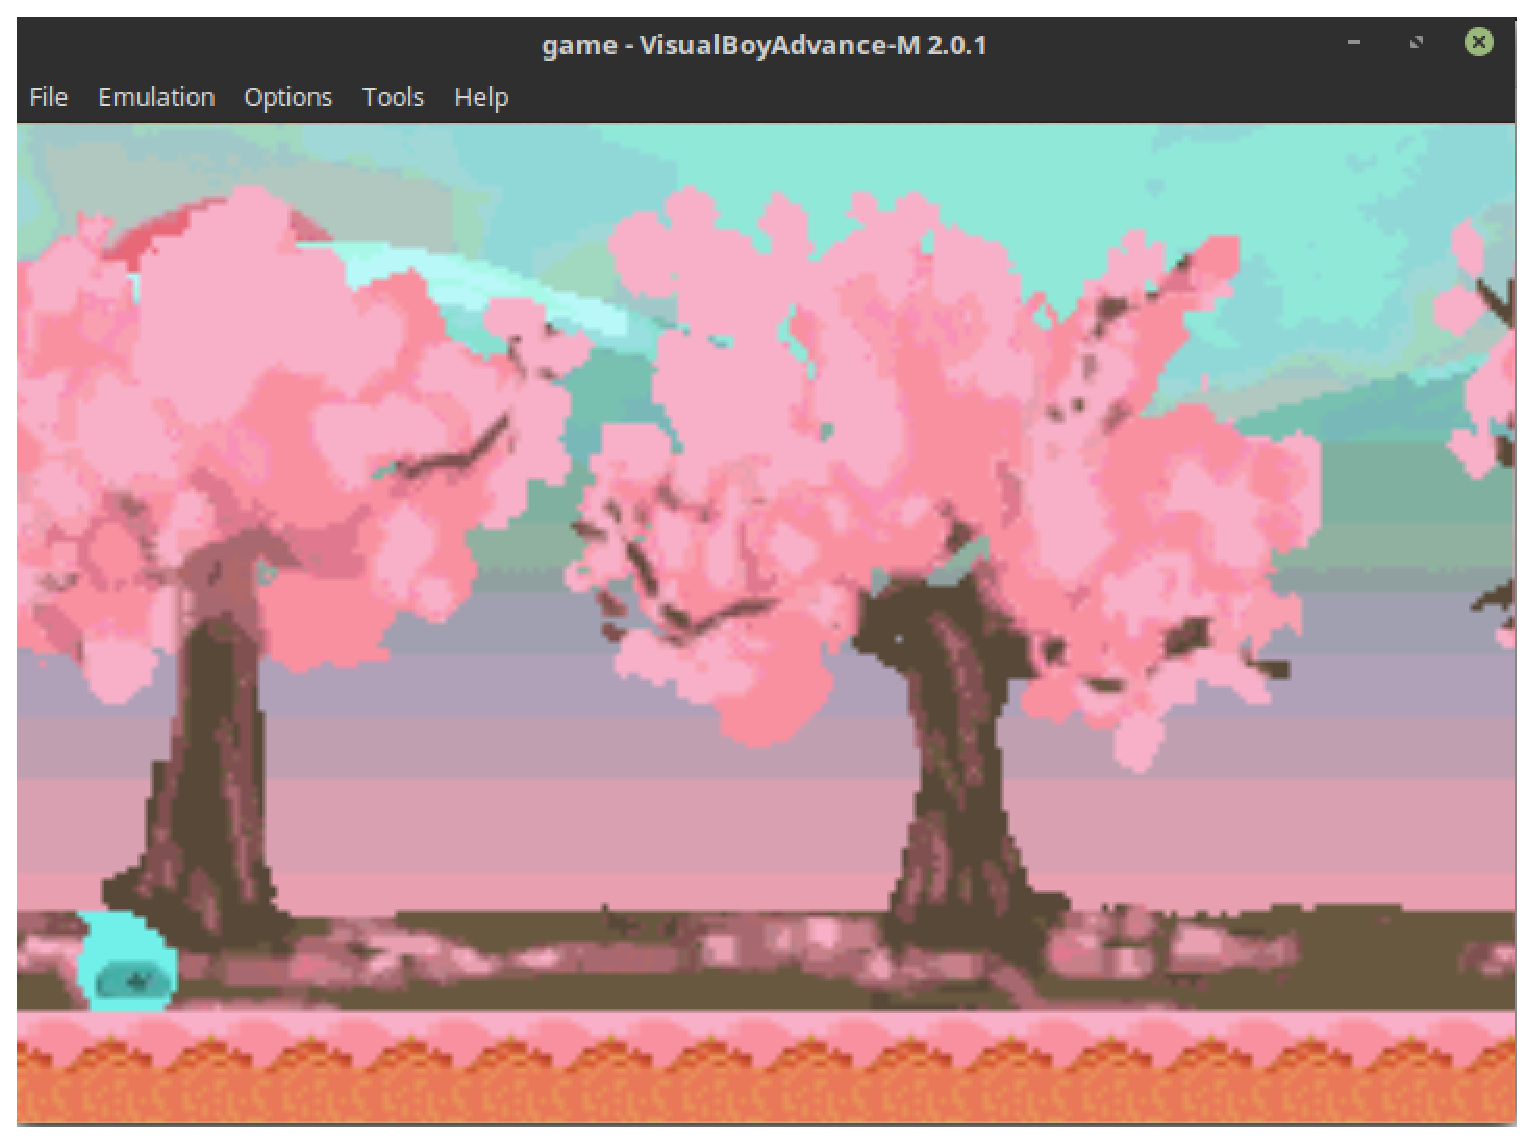
\includegraphics[width=12cm]{figuras/comparacao/gba-fase5.eps} }}%
    \caption{Comparação da quinta fase.}%
    \label{fig:example}%
\end{figure}

\begin{figure}%
    \centering
    \subfloat[Sexta fase original. Fonte: \textit{Autores}.]{{\includegraphics[width=12cm]{figuras/comparacao/pc-fase6.eps} }}%
    \qquad
    \subfloat[Sexta fase portada. Fonte: \textit{Autores}.]{{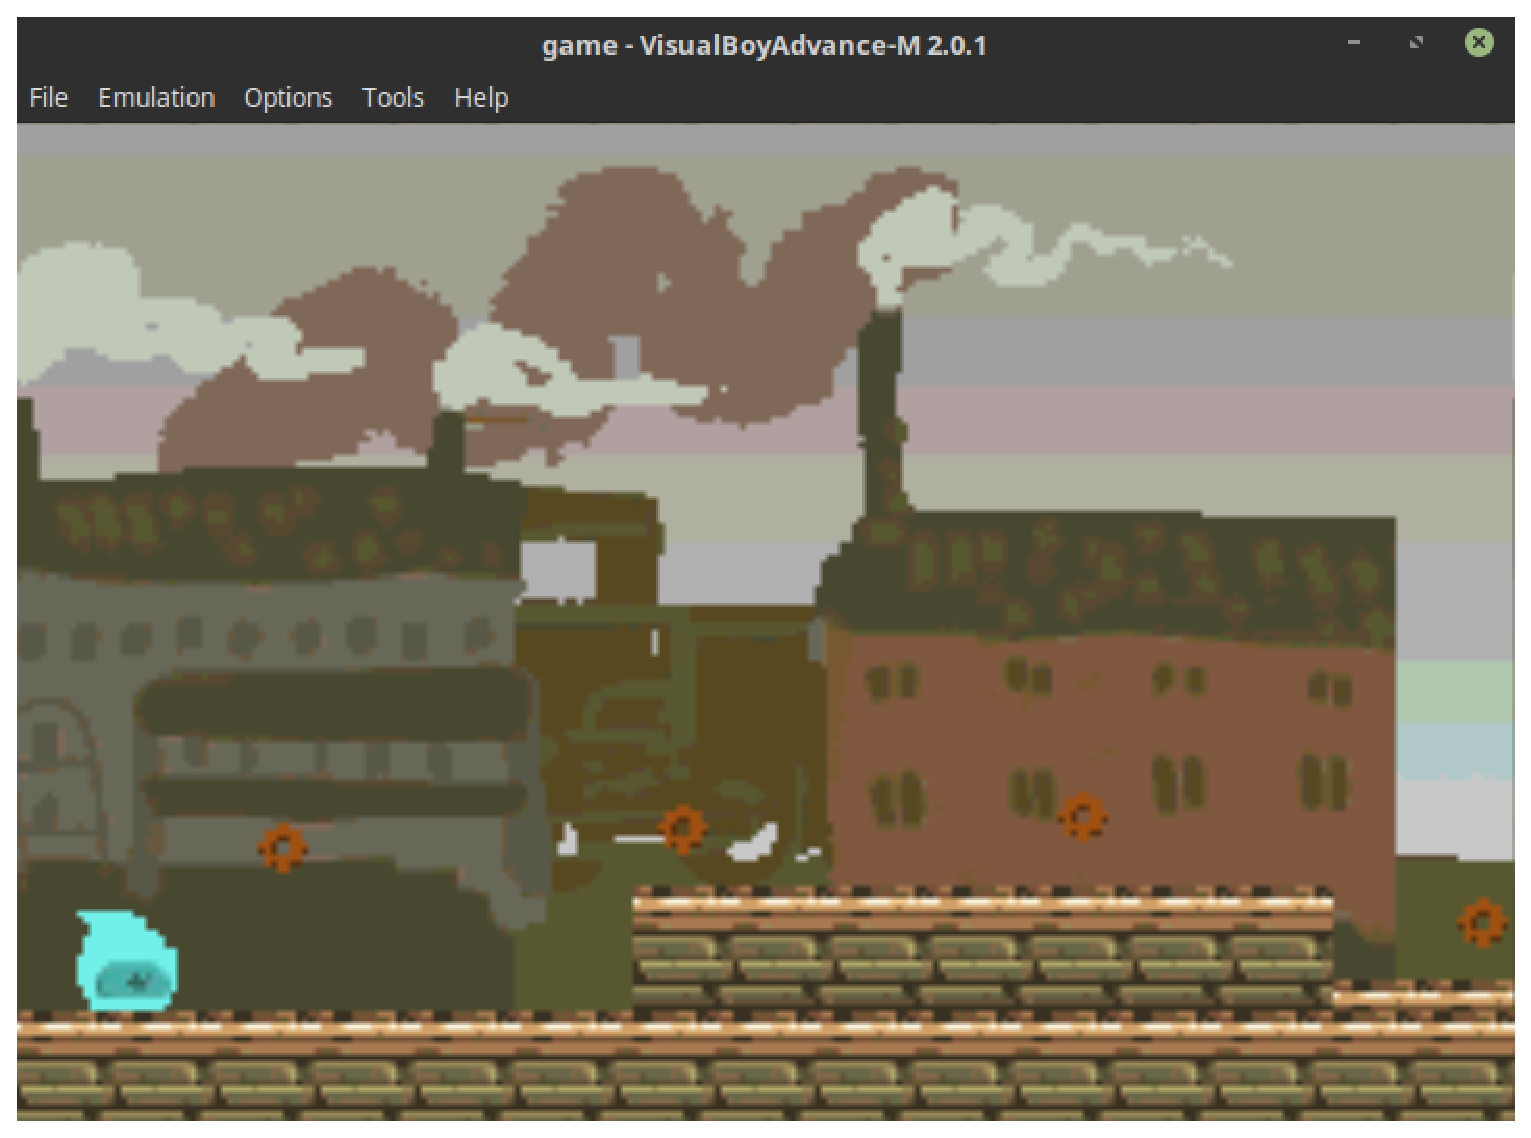
\includegraphics[width=12cm]{figuras/comparacao/gba-fase6.eps} }}%
    \caption{Comparação da sexta fase.}%
    \label{fig:example}%
\end{figure}

\begin{figure}%
    \centering
    \subfloat[Menu de vitória original. Fonte: \textit{Autores}.]{{\includegraphics[width=12cm]{figuras/comparacao/pc-vitoria.eps} }}%
    \qquad
    \subfloat[Menu de vitória portado. Fonte: \textit{Autores}.]{{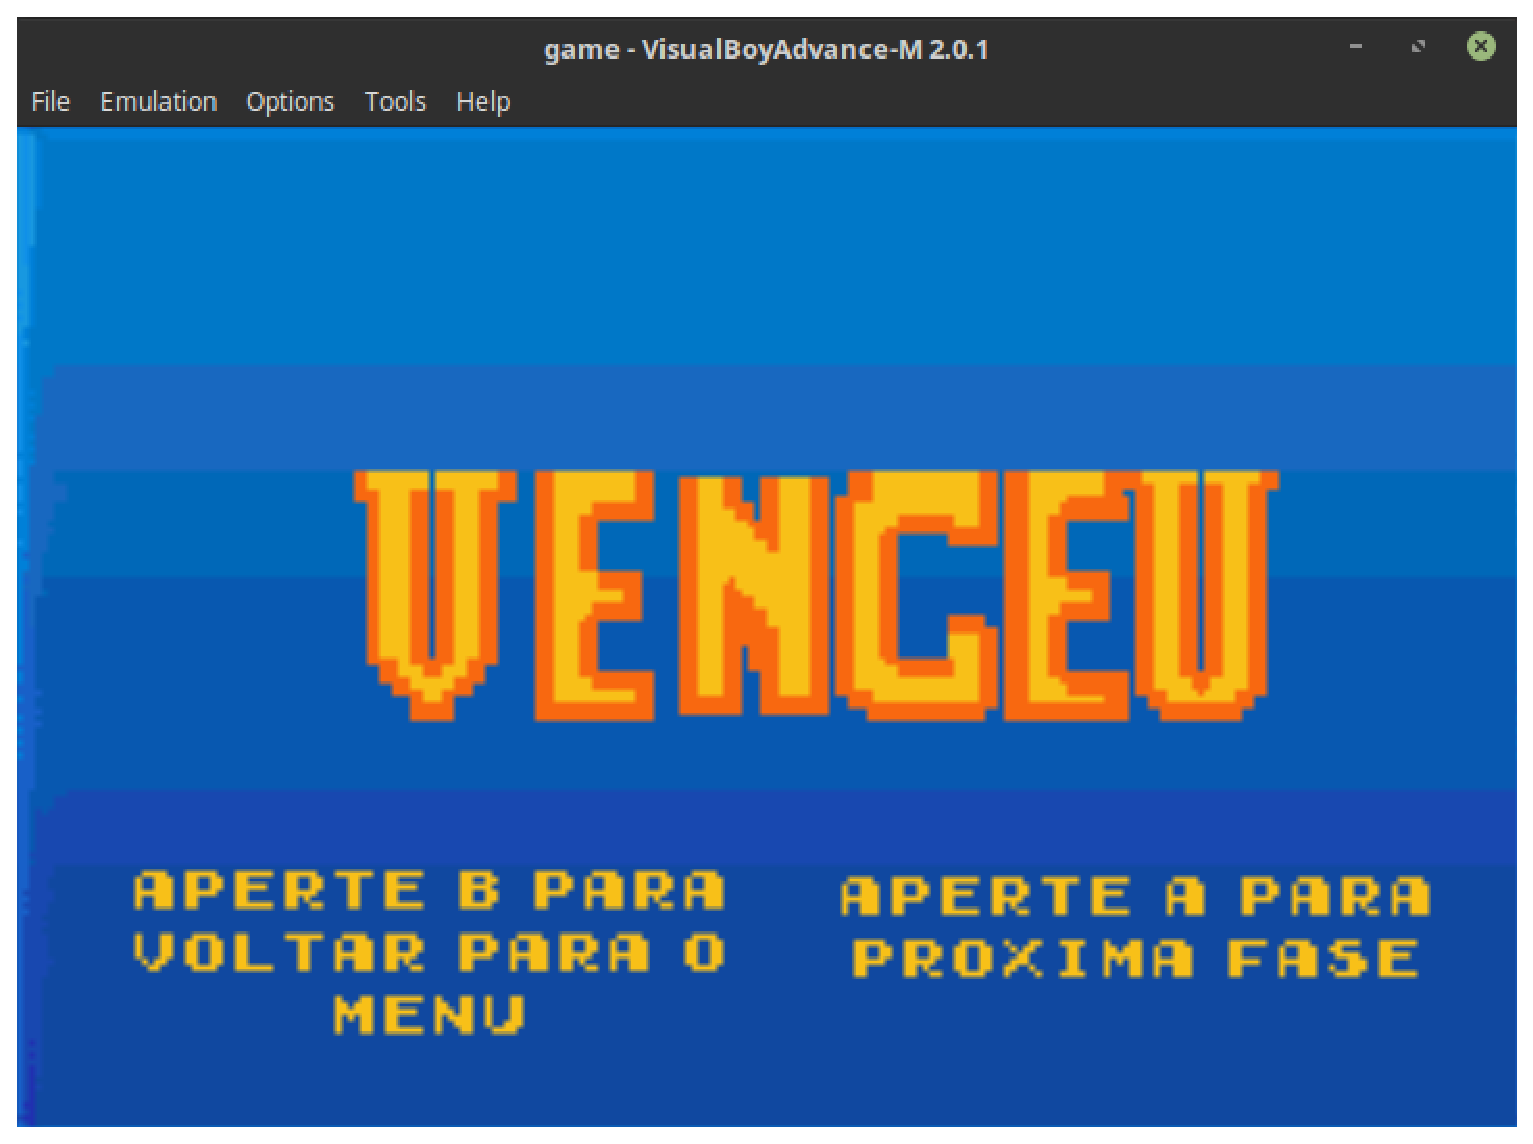
\includegraphics[width=12cm]{figuras/comparacao/gba-vitoria.eps} }}%
    \caption{Comparação do menu de vitória.}%
    \label{fig:example}%
\end{figure}

\begin{figure}%
    \centering
    \subfloat[Menu de derrota original. Fonte: \textit{Autores}.]{{\includegraphics[width=12cm]{figuras/comparacao/pc-defeat.eps} }}%
    \qquad
    \subfloat[Menu de derrota portado. Fonte: \textit{Autores}.]{{\includegraphics[width=12cm]{figuras/comparacao/gba-defeat.eps} }}%
    \caption{Comparação do menu de derrota.}%
    \label{fig:example}%
\end{figure}

% \begin{figure}%
%     \centering
%     \subfloat[Jogo original sendo executado em um PC. Fonte: \textit{Autores}.]{{\includegraphics[width=16cm]{figuras/tw-original-1.eps} }}%
%     \qquad
%     \subfloat[Protótipo sendo executado no emulador de GBA. Fonte: \textit{Autores}.]{{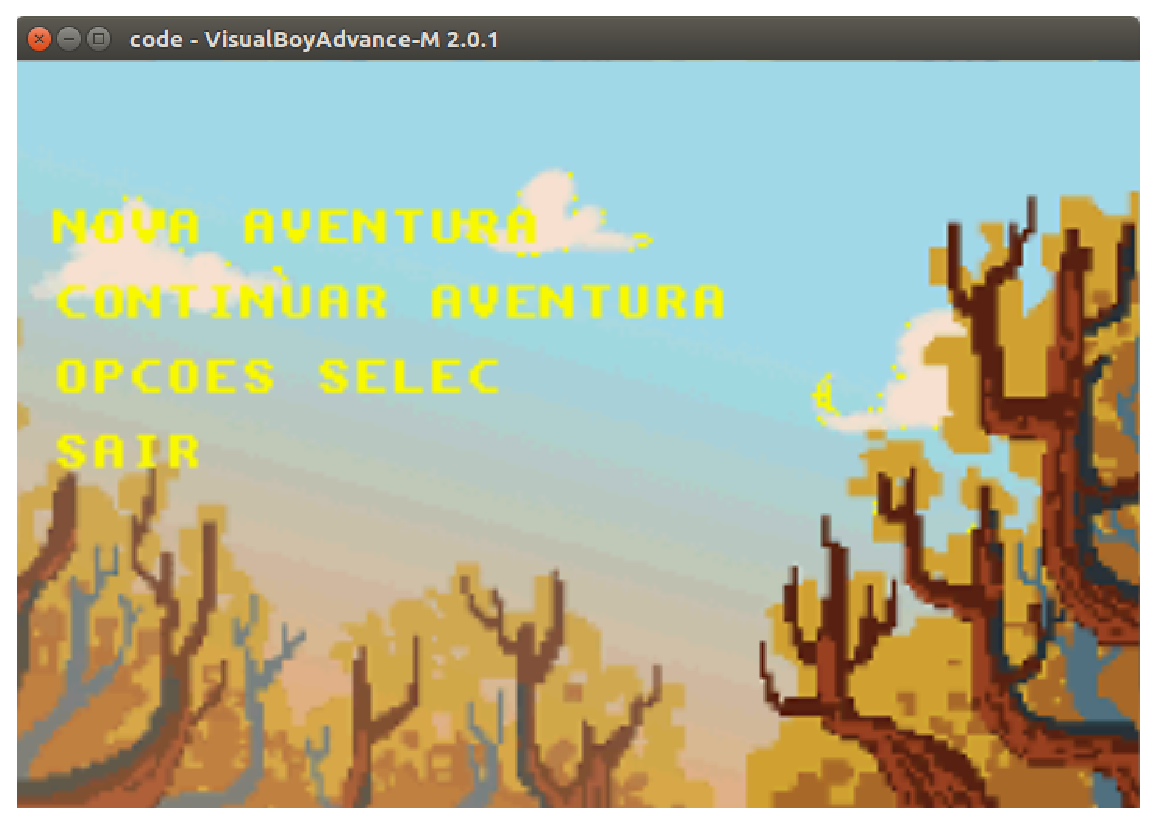
\includegraphics[width=16cm]{figuras/tw-gba-1.eps} }}%
%     \caption{Comparação entre o jogo original e o protótipo no emulador.}%
%     \label{fig:example}%
% \end{figure}